% !TEX root = ../Projektdokumentation.tex
\section{Entwurfsphase} 
\label{sec:Entwurfsphase}

\subsection{Zielplattform}
\label{sec:Zielplattform}
Da es bei diesem Projekt um eine Umsetzung einer Website handelt, wird diese
Applikation auf einem externen Webserver (\ac{HTTP}, Apache2) laufen.
Dementsprechend wird mit der Skriptsprache \ac{PHP} (Version 5.5) gearbeitet. Der Inhalt der Website wird aus
einer MySQL5 Datenbank gespeist.

Neben dem HTML5 wird auch
\ac{CSS}3 und jQuery 1.11.2 -- eine Javascript-Bibliothek für die Umsetzung des
HTML-Dummys eingesetzt. Bei der \mh wird das \ac{CSS} in Form von Less
geschrieben. Less ist eine Stylesheet-Sprache mit dem Ziel, das Schreiben von
CSS zu erleichtern. Dies wird durch intelligente Steuerung und der Vermeidung von 
Code-Wiederholungen bewerkstelligt. Der Less-Code wird anschließend
zu CSS-Code kompiliert.  \footnote{Vgl. Less (Stylesheet-Sprache)
\cite{wiki:Less_(Stylesheet-Sprache)}}

\begin{itemize}
	\item Beschreibung der Kriterien zur Auswahl der Zielplattform (\ua Programmiersprache, Datenbank, Client/Server, Hardware).
\end{itemize}


\subsection{Architekturdesign}
\label{sec:Architekturdesign}
Das \ac{CMS} \ct basiert auf dem \ac{PHP} Web Framework CakePHP (Version 2.8).

CakePHP ist ein freies, open-source-basiertes, rapides Entwicklungsframework für
PHP.
Es ist eine Grundlage für das Programmieren von Web-Applikationen.
Das primäre Ziel ist, in einer strukturierten und rapiden Umgebung zu arbeiten
 -- ohne die Flexiblität zu verlieren.\footnote{Vgl. CakePHP - The Manual
 \cite{CakePHP}}

Wie viele anderen Webframeworks folgt CakePHP dem Schema des
\DesignPattern{\ac{MVC}}. Außerdem sind \ac{DRY}
und \ac{CoC} zugrunde liegende Prinzipien des Frameworks.

Als Basis für das HTML Dummy, wird das CSS-Framework
Bootstrap v.3.3.7 verwendet.
Bootstrap ist ein freies CSS-Framework. Es enthält auf HTML und CSS basierende
Gestaltungsvorlagen für Typografie, Formulare, Buttons, Tabellen, Grid-Systeme, 
Navigations- und andere Oberflächengestaltungselemente sowie zusätzliche, 
optionale JavaScript-Erweiterungen.\footnote{Vgl. Bootstrap
\cite{wiki:Bootstrap_(Framework)}} Neben der Reset-CSS und diversen Fallbacks
für ältere Browser, die keine ausreichende HTML5 Funktionalität aufweisen, stellt Bootstrap Weichen,
\zB zur Optimierung für Touch-Devices, parat. 

\subsubsection{Convention over Configuration}
\label{sec:CoC}
CakePHP versucht, die Konfiguration auf ein Minimum zu beschränken und
spart hiermit viel \\ Arbeitsaufwand. Ein Beispiel wäre die Zuordnung der Models
zu Datenbanktabellen. Dies geschieht über die Namensgleichheit in Singular und Plural. 
Im Detail Model User (Singular) zu Tabelle users (Plural). Der einzige
Konfigurationsschritt ist die Datenbankanbindung selber.


\subsubsection{Model-View-Controller}
\label{sec:MVC}
\ac{MVC} ist ein effektives Entwurfsmuster zur effizienten Umsetzung von 
wartbaren und modularen \\ Webapplikationen. Es gewährleistet eine höhere
Skalierbarkeit und Flexibilität bei Änderungen. Durch die modulare sowie
unterteilte Logik wird es ermöglicht einen Teil der Anwendung zu
verändern, ohne einen anderen Teil zu beeinflussen. Im Folgendem wird eine
simple Darstellung eines \ac{MVC} \begin{figure}[htb] Musters aufgezeigt.
\label{MVC-Diagramm}
\caption{Simples MVC Diagramm}
\center{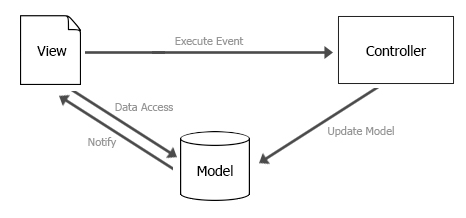
\includegraphics[scale=0.7]{Bilder/mvc.jpg}}
\end{figure}




\subsubsection{7-1 Pattern}
\label{sec:7-1}
Das \DesignPattern{7-1 Pattern}
\footnote{7-1 Pattern, \url{https://www.sass-guidelin.es/#architecture}} ist ein
Muster aus der Frontendarchitektur und definiert sich durch die Strukturierung des \ac{CSS} in 7 Ordner und
einer Hauptdatei. Grundsätzlich sind alle Teile des \ac{CSS} in 7 Ordnern
verteilt, und eine Datei (main.css) die alle Teilstücke importiert und zu einer Stylesheet kompiliert.
\begin{multicols}{4}
\begin{itemize}
\item abstracts/
\item base/
\item components/
\item layout/
\item pages/
\item themes/
\item vendors/
\item main.less
\end{itemize}
\end{multicols}
Die logische und modulare Trennung des \ac{CSS}-Codes verschafft eine klare
Übersicht für den Entwickler. Ebenso wird die Wiederverwendbarkeit von
Teilstücken verbessert und die Skalierbarkeit erhöht. Zusätzlich verschaft man
sich durch die Architektur eine Reihenfolge der Spezifität. Dieses zwingt einen
dazu Spitzen in der Spezifität von Selektoren zu vermeiden oder eher
am Ende des Stylesheets zu platzieren. So befinden sich im zweiten Ordner
"`base/"' nur \ac{CSS}, welches auschließlich HTML Standardelemente (\zB ul,
input,table, \usw) stilisiert. Der nächste Ordner besitzt immer eine höhere
Spezifität als der vorherige. In diesem Fall der Ordner "`components/"', der
bereits Klassen besitzt und aufgrund der höheren Spezifität den Style von
"`base/"' überschreiben kann.




\subsubsection{Block-Element-Modifier}
\label{sec:BEM}
\DesignPattern{Block-Element-Modifier} kurz \acs{BEM} ist ebenso eine moderne
Methode der Frontend-Architektur die erlaubt, Webprojekte modularer zu entwickeln.
Das erleichtert die Wartbarkeit und macht es Entwicklern einfacher, die
Codebasis jederzeit zu erweitern und trotzdem die Übersicht zu behalten.
Code wird in Blöcke und deren Elemente zerlegt, welche sich durch Modifikatoren
verändern lassen. Ein Block kann aus mehreren Elementen bestehen, welche durch
den Modifikator anpassbar sind. Durch dieses einfache Muster ist BEM der ideale
Weg, um im Team an Projekten mit sich ändernden Anforderungen zu arbeiten.
 \footnote{Vgl. t3n - Webdesign Magazin \cite{BEM}}
 
Die Methodik wird im Kapitel \xx chapternr. chaptername anhand eines
praktischen Beispieles naherliegender erläutert.


\begin{itemize}
	\item Beschreibung und Begründung der gewählten Anwendungsarchitektur (\zB \acs{MVC}).
	\item \Ggfs Bewertung und Auswahl von verwendeten Frameworks sowie \ggfs eine kurze Einführung in die Funktionsweise des verwendeten Frameworks.
\end{itemize}


\subsection{Entwurf der Benutzeroberfläche}
\label{sec:Benutzeroberflaeche} 
Das Screendesign wurde von einer externen Werbeagentur zur Verfügung gestellt.
Dementsprechend ist die Durchführung der Corporate Design Richtlinien durch \mh
überflüssig.
Der Screendesigner der \mh hat das Design lediglich in Slices \footnote{Geschnittenen Bilder/Grafiken} 
geschnitten und für die Entwicklung vorbereitet. Zur besseren Übersicht wurde
zusätzlich ein Wireframe gefertigt, welches im \Anhang{app:Entwuerfe}
begutachtet werden kann.


Um dem Entwickler eine bessere Übersicht der nötigen Styles zu bieten, hat der
Screendesigner einen Styleguide entworfen. Dies und weitere Oberflächen sind
ebenfalls unter \Anhang{app:Entwuerfe} zu finden.



\begin{itemize}
	\item Entscheidung für die gewählte Benutzeroberfläche (\zB GUI, Webinterface).
	\item Beschreibung des visuellen Entwurfs der konkreten Oberfläche (\zB Mockups, Menüführung).
	\item \Ggfs Erläuterung von angewendeten Richtlinien zur Usability und Verweis auf Corporate Design.
\end{itemize}


\subsection{Pflichtenheft}
\label{sec:Pflichtenheft}
\begin{itemize}
	\item Auszüge aus dem Pflichtenheft/Datenverarbeitungskonzept, wenn es im Rahmen des Projekts erstellt wurde.
\end{itemize}

\paragraph{Beispiel}
Ein Beispiel für das auf dem Lastenheft (siehe Kapitel~\ref{sec:Lastenheft}: \nameref{sec:Lastenheft}) aufbauende Pflichtenheft ist im \Anhang{app:Pflichtenheft} zu finden.


\Zwischenstand{Entwurfsphase}{Entwurf}
